\section{Auswertung}
\subsection{Sättigungsstrom}
Die gemessenen Daten für einen Heizstrom von $I_f = \SI{2}{\ampere}$ befinden sich in Tab. \ref{tab:20A}, für $I_f = \SI{2.2}{\ampere}$ in Tab. \ref{tab:22A} und für $I_f = \SI{2.4}{\ampere}$ in Tab. \ref{tab:24A}.
\begin{table}
    \centering
    \begin{tabular}{ss}
    \toprule
    U \,/\, \si{\volt}  & I_A \,/\, \si{\milli\ampere} \\
    \midrule
     0 & 0,000 \\
    10 & 0,019 \\
    20 & 0,044 \\
    30 & 0,069 \\
    40 & 0,091 \\
    50 & 0,101 \\
    60 & 0,111 \\
    70 & 0,116 \\
    \bottomrule
    \end{tabular}
    \begin{tabular}{ss}
    \toprule
    U \,/\, \si{\volt}  & I_A \,/\, \si{\milli\ampere} \\
    \midrule
    80 & 0,120 \\
    90 & 0,123 \\
    100 & 0,125 \\
    110 & 0,127 \\
    120 & 0,128 \\
    130 & 0,130 \\
    140 & 0,131 \\
    150 & 0,132 \\
    \bottomrule
    \end{tabular}
    \caption{Der Strom $I_A$ gemessen in Abhängigkeit der angelegten Spannung $U$ für einen Heizstrom von $I_f = \SI{2}{\ampere}$.}
    \label{tab:20A}
\end{table}

\begin{table}
    \centering
    \begin{tabular}{ss}
    \toprule
    U \,/\, \si{\volt}  & I_A \,/\, \si{\milli\ampere} \\
    \midrule
     0 & 0,000 \\
    10 & 0,027 \\
    20 & 0,067 \\
    30 & 0,118 \\
    40 & 0,173 \\
    50 & 0,229 \\
    60 & 0,292 \\
    70 & 0,348 \\
    80 & 0,408 \\
    90 & 0,457 \\
    100 & 0,496 \\
    110 & 0,532 \\
    120 & 0,560 \\
    \bottomrule
    \end{tabular}
    \begin{tabular}{ss}
    \toprule
    U \,/\, \si{\volt}  & I_A \,/\, \si{\milli\ampere} \\
    \midrule
    130 & 0,582 \\
    140 & 0,597 \\
    150 & 0,609 \\
    160 & 0,619 \\
    170 & 0,626 \\
    180 & 0,632 \\
    190 & 0,637 \\
    200 & 0,642 \\
    210 & 0,646 \\
    220 & 0,649 \\
    230 & 0,653 \\
    240 & 0,656 \\
    250 & 0,659 \\
    \bottomrule
    \end{tabular}
    \caption{Der Strom $I_A$ gemessen in Abhängigkeit der angelegten Spannung $U$ für einen Heizstrom von $I_f = \SI{2.2}{\ampere}$.}
    \label{tab:22A}
\end{table}

\begin{table}
    \centering
    \begin{tabular}{ss}
    \toprule
    U \,/\, \si{\volt}  & I_A \,/\, \si{\milli\ampere} \\
    \midrule
     0 & 0,000 \\
     5 & 0,012 \\
    10 & 0,028 \\
    15 & 0,048 \\
    20 & 0,072 \\
    25 & 0,098 \\
    30 & 0,131 \\
    35 & 0,169 \\
    40 & 0,207 \\
    45 & 0,248 \\
    50 & 0,289 \\
    55 & 0,336 \\
    60 & 0,382 \\
    70 & 0,476 \\
    80 & 0,578 \\
    90 & 0,673 \\
    \bottomrule
    \end{tabular}
    \begin{tabular}{ss}
    \toprule
    U \,/\, \si{\volt}  & I_A \,/\, \si{\milli\ampere} \\
    \midrule
    100 & 0,774 \\
    110 & 0,918 \\
    120 & 1,025 \\
    130 & 1,126 \\
    140 & 1,229 \\
    150 & 1,337 \\
    160 & 1,432 \\
    170 & 1,538 \\
    180 & 1,632 \\
    190 & 1,717 \\
    200 & 1,807 \\
    210 & 1,892 \\
    220 & 1,971 \\
    230 & 2,05 \\
    240 & 2,12 \\
    250 & 2,18 \\
    \bottomrule
    \end{tabular}
    \caption{Der Strom $I_A$ gemessen in Abhängigkeit der angelegten Spannung $U$ für einen Heizstrom von $I_f = \SI{2.4}{\ampere}$.}
    \label{tab:24A}
\end{table}
\FloatBarrier
Im Sättigungsstromgebiet kann die Kurve durch die Funktion
\begin{equation}
    I(U) = I_S - A \cdot \mathrm{e}^{-B \cdot U}
    \label{eqn:ausgleich}
\end{equation} 
angenähert werden.
Aus einer Ausgleichsrechnung \cite{scipy} mit der Funktion \ref{eqn:ausgleich} für das Sättigungsstromgebiet folgt der Sättigungsstrom $I_S$ (siehe Tab. \ref{tab:saettigungsstrom}).
\begin{table}
    \centering
    \begin{tabular}{c|cc}
        \toprule
        $I_f \,/\, \si{\ampere}$ & $\text{Anfang Sättigungsgebiet } U_A \,/\, \si{\volt}$ & $I_S \,/\, \si{\milli\ampere}$ \\
        \midrule
        $2.0$ & $20$ & $\SI{131.2(7)}{}$ \\
        $2.2$ & $60$ & $\SI{664.8(22)}{}$ \\
        $2.4$ & $110$ & $\SI{4250(180)}{}$ \\
        \bottomrule
    \end{tabular}
    \caption{Der durch eine Ausgleichsrechung ermittelte Sättigungsstrom $I_S$ für einen bestimmten Heizstrom $I_f$.}
    \label{tab:saettigungsstrom}
\end{table}
In Abb. \ref{fig:kurvenchar} ist der gemessene Strom in Abhängigkeit der Spannung und ein Fit für das Sättigungsstromgebiet aufgetragen.
\begin{figure}
    \centering
    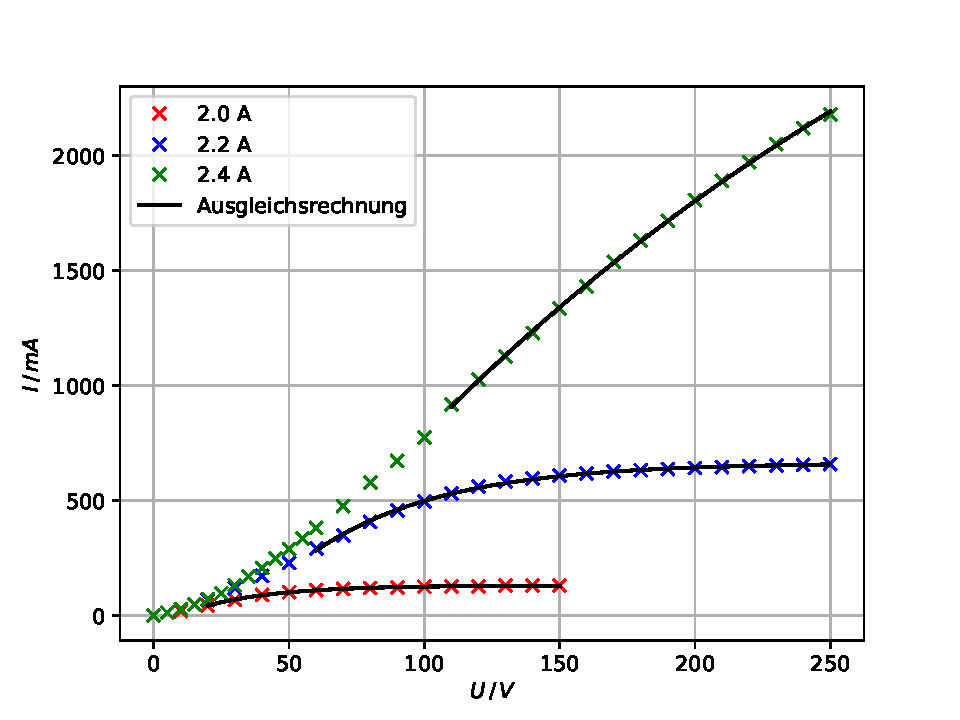
\includegraphics[width=0.8\textwidth]{content/data/saettigungsstrom.pdf}
    \caption{Der gemessene Strom $I_A$ und eine Ausgleichskurve für die drei Heizströme.\cite{matplotlib}\cite{numpy}\cite{scipy}\cite{uncertainties}}
    \label{fig:kurvenchar}
\end{figure}
\FloatBarrier

\subsection{Langmuir-Schottkysche Raumladungsgesetz}
Hier wird nur das Raumladungsgebiet bei maximalen Heizstrom $I_f = \SI{2.4}{\ampere}$ (siehe Tab. \ref{tab:20A}) betrachtet.
Das Raumladungsgebiet liegt im Intervall $\left [ \SI{0}{\volt}, \SI{60}{\volt} \right ]$ und kann durch das Langmuir-Schottkysche Raumladungsgesetz beschrieben werden. %ref
Der Exponent $b$ der Strom-Spannung Beziehung wird durch eine Ausgleichrechnung \cite{scipy} der Form
\begin{equation*}
    I(U) = a \cdot U^b
\end{equation*}
ermittelt.
Daraus folgt für die Parameter:
\begin{align*}
    a &= \SI{7.55(32)e-7}{} \\
    b &= \SI{1.521(11)}{}
\end{align*}
Die Messwerte im Raumladungsgebiet und der zugehörige Fit sind in Abb. \ref{fig:langmuir} graphisch dargestellt.
\begin{figure}
    \centering
    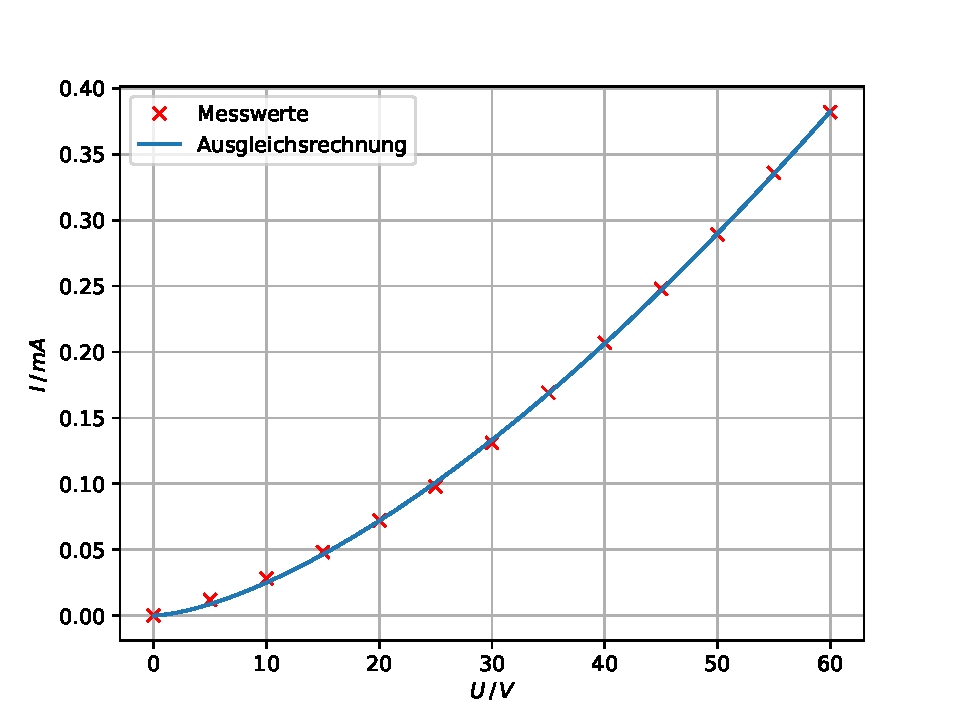
\includegraphics[width=0.8\textwidth]{content/data/langmuir.pdf}
    \caption{Das Raumladungsgebiet bei einem Heizstrom von $I_f = \SI{2.4}{\ampere}$ mit einer Ausgleichskurve dargestellt. \cite{scipy}\cite{numpy}\cite{matplotlib}}
    \label{fig:langmuir}
\end{figure}
\FloatBarrier

\subsection{Anlaufstromgebiet}
Im folgenden wird das Anlaufstromgebiet untersucht.
In Tab. \ref{tab:anlauf} befindet sich der gemessene Anlaufstrom $I$ in Abhängigkeit der Bremsspannung $U$ für die maximale Heizleistung $I_f = \SI{2.4}{\ampere}$.
Zumdem muss die Spannung, wegen des Innenwiderstand $R_i = \SI{1}{\mega\ohm}$ nach der Gleichung
\begin{equation}
    U_K = U - R_i \cdot I
\end{equation}
korrigiert werden (siehe Tab. \ref{tab:anlauf}).
\begin{table}
    \centering
    \begin{tabular}{ccc}
        \toprule
        $U \,/\, \si{\volt}$ & $I \,/\, \si{\nano\ampere}$ & $U_K \,/\, \si{\volt}$ \\
        \midrule
        $0.0$ & $8$ & $-0.008$ \\
        $0.1$ & $4$ & $0.0096$ \\
        $0.2$ & $2$ & $0.198$ \\
        $0.3$ & $1.75$ & $0.298$ \\
        $0.4$ & $0.8$ & $0.399$ \\
        $0.5$ & $0.5$ & $0.500$ \\
        $0.6$ & $0.25$ & $0.600$ \\
        $0.7$ & $0.21$ & $0.700$ \\
        $0.8$ & $0.15$ & $0.800$ \\
        $0.9$ & $0.10$ & $0.900$ \\
        \bottomrule
    \end{tabular}
    \caption{Der gemessene Strom $I$ in Abhängigkeit der Spannung $U$ und die korrigierte Spannung $U_K$.}
    \label{tab:anlauf}
\end{table}
Nun wird mit der korrigierten Spannung $U_K$ und dem Strom $I$ eine Ausgleichrechnung \cite{scipy} nach Gleichung durchgeführt %ref
Daraus folgt die Temperatur $T$ der Glühkathode
\begin{equation*}
    T = \SI{1950(10)}{\kelvin} \, .
\end{equation*}
Die Messwerte und der Fit sind in Abb. \ref{fig:anlauf} graphisch dargestellt.
\begin{figure}
    \centering
    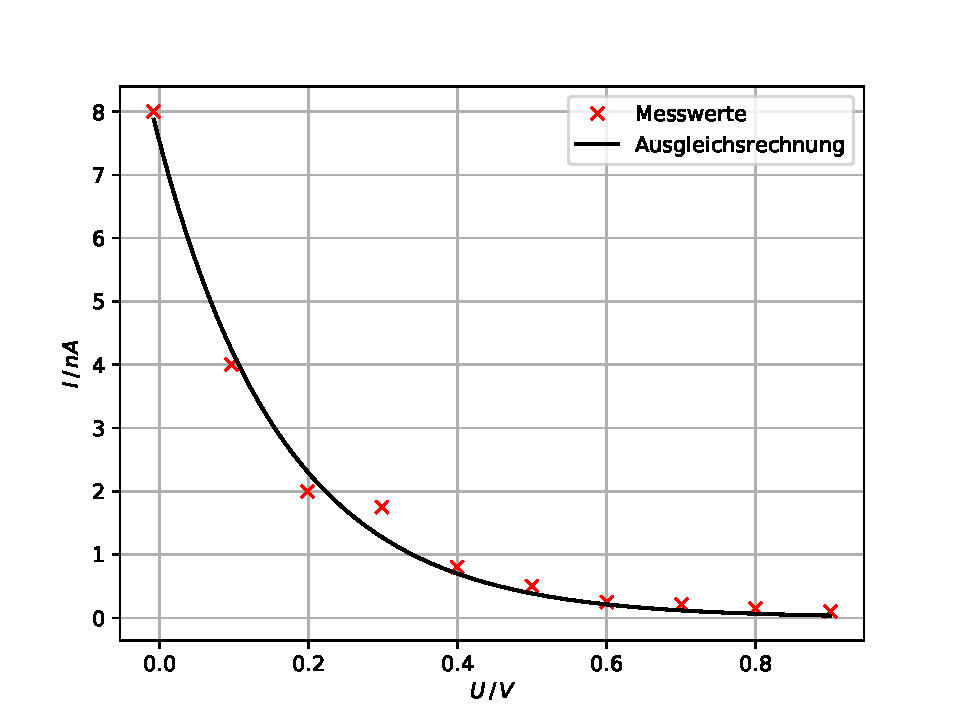
\includegraphics[width=0.8\textwidth]{content/data/anlaufgebiet.pdf}
    \caption{Das Anlaufgebiet bei maximalen Heizstrom $I_f=\SI{2.4}{\ampere}$ mit einer Ausgleichskurve. \cite{scipy}\cite{numpy}\cite{matplotlib}}
    \label{fig:anlauf}
\end{figure}
\FloatBarrier

\subsection{Leistungsbilanz des Heizstromkreises}
Als nächstes wird die Kathodentemperatur $T$ durch die Gleichung %ref
\begin{equation*}
    \sqrt[4]{\frac{I_f U_f - N_{WL}}{f \eta \sigma}}
\end{equation*}
ermittelt.
In Tab. \ref{tab:leistung} befinden sich die Spannungs- und Stromwerte für den Heizkreis und die daraus folgende Temperatur.
$N_{WL}$ beträgt schätzungsweise $\SI{1}{\watt}$.
Weitere Konstanten werden der Versuchsanleitung \cite{anleitung} entnommen.
\begin{table}
    \centering
    \begin{tabular}{sss}
        \toprule
        I_f \,/\, \si{\ampere} & U_f \,/\, \si{\volt} & T \,/\, \si{\kelvin} \\
        \midrule
        2,0 & 4,0 & 1881,48 \\
        2,2 & 4,5 & 1997,89 \\
        2,4 & 5,5 & 2161,80 \\
        \bottomrule
    \end{tabular}
    \caption{Die ermittelte Temperatur $T$ bei konstantem Heizstrom $I_f$ und -spannung $U_f$.}
    \label{tab:leistung}
\end{table}
\FloatBarrier

\subsection{Austrittsarbeit der Elektronen}
Mithilfe der Richardson-Gleichung%ref
\begin{equation*}
    \phi = -\frac{k_B T}{e_0} \ln \left( \frac{I_S h^3}{4\pi f e_0 m_0 k_B^2 T^2}  \right)
\end{equation*}
kann die Austrittsarbeit $\phi$ der Elektronen bestimmt werden.
Die Konstanten werden der Literatur \cite{konstanten} entnommen.
In Tab. \ref{tab:austrittsarbeit} befinden sich die berechneten Austrittsarbeiten $\phi$.
\begin{table}
    \centering
    \begin{tabular}{cc}
        \toprule
        $I_f \,/\, \si{\ampere}$ &  $\phi \,/\, \si{\electronvolt}$ \\
        \midrule
        $2.0$ & $\SI{3.7538(9)}{}$ \\
        $2.2$ & $\SI{3.7273(6)}{}$ \\
        $2.4$ & $\SI{3.7170(80)}{}$ \\
        \bottomrule
    \end{tabular}
    \caption{Die ermittelte Austrittsarbeit $\phi$ bei konstantem Heizstrom $I_f$.}
    \label{tab:austrittsarbeit}
\end{table}
\FloatBarrier
Im Mittel beträgt die Austrittsarbeit
\begin{equation*}
    \bar{\phi} = \SI{3.7327(27)}{\electronvolt} \, .
\end{equation*}